\documentclass[fleqn]{jbook}
\usepackage{physpub}

\begin{document}

\begin{question}{専攻 問題1}{}

\begin{subquestions}
\SubQuestion
  右図のように$0<x<d$で$U(x)=U_0$、それ以外は$U(x)=0$であるような
  一次元のポテンシャルの壁に、左側の無限遠から質量$m$、エネルギー
  $E=U_0/2$の粒子が入射するものとして、以下の問に答えよ。
%
  \begin{subsubquestions}
  \vspace*{-5mm}\parbox[t]{98mm}{
  \SubSubQuestion
    一般に、有界な1次元のポテンシャルの不連続点で波動関数が満たすべき
    条件をあげ、その理由を述べよ。

  \SubSubQuestion
    右図の条件に対応する波動関数の領域$x\leq 0$における形を
%
    \[ \psi=e^{ikx}+\beta e^{-ikx} \hspace{10mm} \mbox{ここで}%
       k=\frac{1}{\hbar}\sqrt{2mE} \]
%
    とする。$\beta$は未知係数である。同様に、$0<x<d,d\leq x$における
    波動関数をそれぞれ適当な未知係数を用いて表せ。
  }\parbox[t]{58mm}{
  \begin{center}\vspace*{5mm}
    \mbox{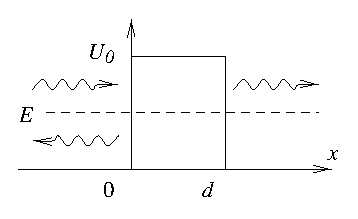
\includegraphics[clip]{1994phy1-1.eps}}
  \end{center}}

  \SubSubQuestion
    透過率を$T$とする。次式を示せ。
%
    \begin{equation}
      T=\frac{1}{\sinh^2(kd)+1} \eqname{1}
    \end{equation}

  \end{subsubquestions}

\SubQuestion
  WKB法の近似によれば、右図のような1次元の滑らかなポテンシャル障壁
  $U(x)$に左側の無限遠から質量$m$、エネルギー$E$の粒子が入射するもの
  として、透過率$T$は$T\ll 1$の場合
%
  \begin{equation}
    T\simeq \exp\left[-2\int_a^bq(x)\d{x}\right] \hspace{10mm}%
    q(x) = \frac{1}{\hbar}\sqrt{2m(U(x)-E)}   \eqname{2}
  \end{equation}
%
  で与えられる。以下の問に答えよ。
%
  \begin{subsubquestions}
  \vspace*{-5mm}\parbox[t]{98mm}{
  \SubSubQuestion
    設問{\bf 1}のポテンシャルは滑らかでないが、$T \ll 1$の場合は
    式\eqhref{1}の$T$は数係数を除きWKB法の近似式\eqhref{2}
    と一致することを示せ。
  }\parbox[t]{56mm}{\vspace*{-12mm}
  \begin{center}
    \mbox{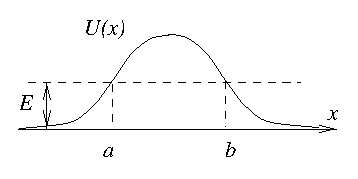
\includegraphics[clip]{1994phy1-2.eps}}
  \end{center}}

  \SubSubQuestion
    金属の表面に強い電場を加えると電子が放出される現象を電界放出と
    いう。電界放出による電流密度$j$と電場$F$の間には、左下の図に示す
    ような関係があることが知られている。
    この現象の簡単なモデルとして、
    $x=0$を金属の表面、$x<0$を金属の内部とし、電子に対するポテンシャル
    を右下の図に示すように$x<0$で$U(x)=0$、$0\leq x$で$U(x)=U_1-eFx$と
    する。ここで、$e$は電子の電荷の絶対値である。金属内部で電子は一定
    のエネルギー$E\;(0<E<U_1)$をもち、$x$軸と平行に運動するものとする。
    電子の質量を$m$とし、WKB法の近似式\eqhref{2}を用いて透過率を求め、
    電流密度は透過率に比例するとして、左下の図の関係を説明せよ。
  \end{subsubquestions}
  \begin{center}
    \mbox{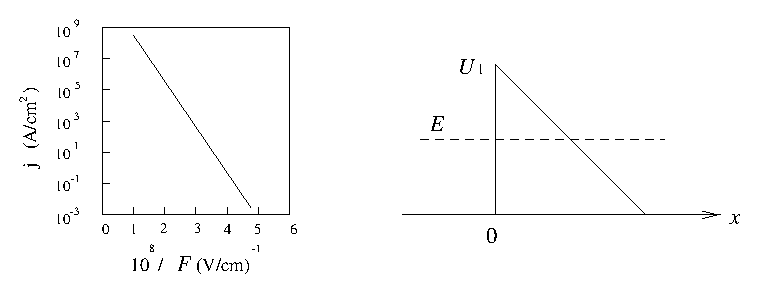
\includegraphics[clip]{1994phy1-3.eps}}
  \end{center}
\end{subquestions}
\end{question}
\begin{answer}{専攻 問題1}{}

\begin{subanswers}
\SubAnswer
  \begin{subsubanswers}
  \SubSubAnswer
    Schr\"{o}dinger方程式
%
    \[ \left[\frac{-\hbar ^2}{2m}\Partial{^2\psi (x)}{x^2}+U(x)\right]
       \psi (x)=E\psi (x)\]
%
    より、$\Partial{^2\psi (x)}{x^2}$は明らかにpotentialの不連続点
    $x=x_0$で不連続。\\
    Schr\"{o}dinger方程式を、potentialの不連続点$x=x_0$の近傍
    $\left[ {x_0-\delta_2 \,,\, x_0+\delta_1 } \right]$
    で積分すると、
%
    \[ \frac{-\hbar ^2}{2m}\int_{x_0-\delta_2}^{x_0+\delta_1} 
       \Partial{^2\psi (x)}{x^2}\d{x}
      +\int_{x_0-\delta_2}^{x_0+\delta_1} {\left[ {U(x)-E} \right]\psi (x)\d{x}}=0 \]
%
    で、potential $U(x)$は有界だから、左辺第2項
    $=O(\delta_1)+O(\delta_2)$、$\delta_1,\delta_2 \rightarrow +0$
    で$\rightarrow 0$である。したがって
%
    \[\left[ \Partial{\psi}{x} \right]_{x_0-\delta_2 }^{x_0+\delta_1 }=O(\delta)\]
%
    すなわち、$\delta_1,\delta_2 \rightarrow +0$の極限で、
%
    \[ \left. \Partial{\psi }{x}\right|_{x_0+0 }=
       \left. \Partial{\psi }{x} \right|_{x_0-0 }\]
%
    が必要。\\
    また波動関数を確率的に解釈するために波動関数の連続性
%
    \[\psi (x_0+0 )=\psi (x_0-0 )\]
%
    が必要。

  \SubSubAnswer
    領域$0<x<d$ではSchr\"{o}dinger方程式は、
%
    \[ \Partial{^2\psi (x)}{x^2}%
         = -\frac{2m}{\hbar ^2}(E-U_0)\psi (x)%
         =  \frac{mU_0}{\hbar ^2}\psi (x)=k^2\psi (x) \]
%
    だから、波動関数は未知係数$A$,$B$を用いて
%
    \[ \psi (x)=Ae^{kx}+Be^{-kx} \]
%
    と書ける。

    領域$x>d$ではSchr\"{o}dinger方程式は、
%
    \[ \Partial{^2\psi (x)}{x^2}=-{\frac{2m}{\hbar ^2}}E\psi (x)
       = -{\frac{mU_0}{\hbar ^2}}\psi (x)=-k^2\psi (x)\]
%
    だから、波動関数は未知係数$C$を用いて
%
    \[ \psi (x)=Ce^{ik(x-d)}\]
%
    と書ける。$e^{-ikx}$の項は$x=\infty $から$x$のマイナス方向への
    進行波なので物理的考察から排除される。

  \SubSubAnswer
    currentは
%
    \[ j = \frac{1}{m}{\rm Re} \left(%
            {\psi ^*(-i\hbar \Partial{}{x})\psi } \right)\]
%

    で与えられるので、
%
    \[ \psi _{\rm in}=e^{ikx}, \quad%
       \psi _{\rm ref}=\beta e^{-ikx}, \quad%
       \psi _{\rm tr}=Ce^{ik(x-d)} \]
%
    を用いて計算すると、透過率は
%
    \[ \frac{j_{tr}}{j_{in}}=\left| C \right|^2 \]
%
    で与えられる。

    さてここで、$x=0$と$x=d$での境界条件から、
%
    \begin{eqnarray*}
      1+\beta &=&A+B \\
      i(1-\beta )&=&A-B \\
      Ae^{kd}+Be^{-kd}&=&C\\
      Ae^{kd}-Be^{-kd}&=&iC
    \end{eqnarray*}
%
    である。これらの4つの変数についての4つの式を、$\beta,C$について
    解くと
%
    \[ \beta = -i{\rm tanh} (kd) \hspace{10mm}%
       C = {\rm sech} (kd) = \frac{1}{{\rm cosh}(kd)}\]
%
    である。

    したがって、透過率$T$は
%
    \[ T={\rm cosech}^2(kd)=\frac{1}{\sinh ^2(kd)+1} \]
%
    である。

  \end{subsubanswers}

\SubAnswer
  \begin{subsubanswers}
  \SubSubAnswer
    近似式\eqhref{2}で透過率を求めると
%
    \[ T \cong \exp \left[ -2\int_0^d \frac{\d{x}}{\hbar}%
               \sqrt{2m\left( U_0-\frac{U_0}{2} \right)}\; \right]%
         = \exp \left[-2\int_0^d\frac{\d{x}}{\hbar}\sqrt{2m E}\; \right]%
         = \exp \left[ -2\int_0^d k \d{x} \right]%
         = e^{-2kd} \]
%
    である。

    一方、$1\ll kd$のとき
%
    \[ 1\ll \cosh ^2(kd)\cong \frac{e^{2kd}}{4} \]
%
    であるから、設問{\bf 1}で求めた透過率は
%
    \[4e^{-2kd}\]
%
    である。

  \SubSubAnswer
    電子のポテンシャル
%
    \[ U(x) = \left\{\begin{array}{lc}%
             \ds  0       & (x<0) \\
             \ds  U_1-eFx & (x>0) \end{array}\right. \]
%
    ($U_1$:金属の仕事関数;F:電界)\\
    エネルギーE\,$(<U_1)$の金属内電子がトンネル効果で抜ける必要のある
    場所は$x=0$から$x=\frac{U_1 - E}{eF}$までである。
%
    \begin{eqnarray*}
      T &\cong& \exp \left[-2\int_0^{\frac{U_1-E}{eF}}\frac{\d{x}}{\hbar}
               \sqrt{2m(U_1-eFx-E)} \right]\\
        &=& \exp \left[ -\frac{2}{\hbar}\left[-\frac{2}{3}%
                 {(2m(U_1-E-eFx))}^\frac{3}{2}\frac{1}{2meF}%
                 \right]_0^{\frac{U_1-E}{eF}} \right]\\
        &=& \exp \left[ -\frac{2}{3m\hbar eF}\left\{{2m(U_1-E)}%
                 \right\}^{3/2}\right]
    \end{eqnarray*}
%
    だから、
%
    \[ \log_{10}j=\log_{10}T+{\rm const}=\frac{1}{\ln 10}\left[%
      -\frac{2}{3m\hbar eF}\left\{ 2m(U_1-E) \right\}^{3/2}%
       \right] + {\rm const} \]
%
    で、$1/F$に比例してさがる。これはグラフの結果と一致する。

  \end{subsubanswers}
\end{subanswers}
\end{answer}


\end{document}
